\documentclass[t]{beamer}
\usepackage[utf8]{inputenc}  % to be able to type unicode text directly
\usepackage{inconsolata}     % for a nicer (e.g. non-courier) tt family font
\usepackage{array}           % to fine-tune tabular spacing
\usepackage{bbm}             % for blackboard 1
\usepackage{graphicx}        % to include images
\usepackage{graphbox}       % to fine-tune image alignment
%\usepackage{animate}         % to include animated images
\usepackage{soul}            % for colored strikethrough
%\usepackage{bbding}          % for Checkmark and XSolidBrush
\usepackage{hyperref,url}

\colorlet{darkgreen}{black!50!green}  % used for page numbers
\colorlet{darkred}{black!50!red}  % used for page numbers
\colorlet{darkblue}{black!30!blue}  % used for page numbers
\colorlet{lightblue}{white!50!blue}  % used for page numbers
\definecolor{term}{rgb}{.9,.9,.9}     % used for code insets

\setlength{\parindent}{0em}  % no paragraph indentation
\setlength{\parskip}{1em}    % paragraph spacing


% coco's macros
\def\R{\mathbf{R}}
\def\F{\mathcal{F}}
\def\x{\mathbf{x}}
\def\y{\mathbf{y}}
\def\u{\mathbf{u}}
\def\Z{\textbf{Z}}
\def\d{\mathrm{d}}
\newcommand{\Abs}[1]{\left\| #1 \right\|}
\DeclareMathOperator*{\argmin}{arg\,min}
\DeclareMathOperator*{\argmax}{arg\,max}
\newcommand{\reference}[1] {{\scriptsize \color{gray}  #1 }}
\newcommand{\referencep}[1] {{\tiny \color{gray}  #1 }}
\newcommand{\unit}[1] {{\tiny \color{gray}  #1 }}

% disable spacing around verbatim
\usepackage{etoolbox}
\makeatletter\preto{\@verbatim}{\topsep=0pt \partopsep=0pt }\makeatother

% disable headings, set slide numbers in green
\mode<all>\setbeamertemplate{navigation symbols}{}
\defbeamertemplate*{footline}{pagecount}{\leavevmode\hfill\color{darkgreen}
   \insertframenumber{} / \inserttotalframenumber\hspace*{0ex}\vskip0pt}

%% select red color for strikethrough
\makeatletter
\newcommand\SoulColor{%
  \let\set@color\beamerorig@set@color
  \let\reset@color\beamerorig@reset@color}
\makeatother
\newcommand<>{\St}[1]{\only#2{\SoulColor\st{#1}}}
\setstcolor{red}

% make everything monospace
\renewcommand*\familydefault{\ttdefault}





\begin{document}


\addtocounter{framenumber}{-1}
\begin{frame}[plain,fragile]
\Large
\begin{verbatim}






  the Riesz semigroup in image processing






mnhrdt
gtti 6/4/2023
\end{verbatim}
\end{frame}



% intro 1 newton vs. others
\begin{frame}
INTRO\\
=====

{\bf Question:}
Who is the best scientist of all time?

\pause
{\bf Answer:}
Easy! It's Isaac Newton

\pause
\vfill

{\bf Question:}
Who is the {\color{blue} second-best} scientist of all time?

\pause
{\bf Answer:}
Hmmm...\\
\color{blue}
\small
Archimedes, von Neumann, Einstein, Darwin, Pasteur,
Curie, Galileo, Lavoisier, Maxwell, $\ldots$

\end{frame}

% intro 2 gaussian kernel vs. riesz kernel
\begin{frame}
INTRO\\
=====

{\bf Question:}
%\\
What is the best convolution kernel?\\
\pause
{\bf Answer:}
Easy! The Gaussian kernels
%\[
%	\color{darkblue}
%	G_\sigma(x,y)\ =\  {\color{lightblue}\frac1{2\pi\sigma^2}} \exp\frac{-(x^2+y^2)}{2\sigma^2}
%	\pause
%	\ =\  {\color{lightblue}\frac1{\sigma^d\sqrt{2\pi}^d}}
%	\exp\frac{-\Abs{\vec x}^2}{2\sigma^2}
%\]
\begin{tabular}{ll}
	\fbox{
		\(\displaystyle\color{darkblue}
	G_\sigma(x,y)\ =\  {\color{lightblue}\frac1{2\pi\sigma^2}} \exp\frac{-(x^2+y^2)}{2\sigma^2}
		\)
	}&
	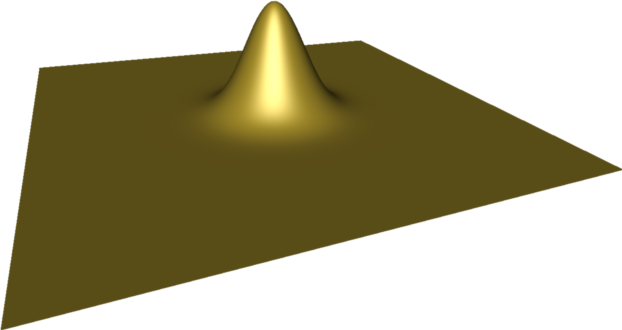
\includegraphics[align=c,width=0.29\textwidth]{f/shot_gauss.png}
\end{tabular}

\pause
%\vfill

{\bf Question:}
What is the second-best convolution kernel?\\
\pause
{\bf Answer:}
Easy! The Riesz potentials:
%\[
%	\color{darkred}
%	R_\sigma(x,y)\ =\  {\color{pink}k_\sigma}
%	\left(x^2+y^2\right)^{\frac{\sigma-2}2}
%	\pause
%	\ =\  {\color{pink}k_\sigma}
%	\frac1{\Abs{\vec x}^{d-\sigma}}
%\]
\begin{tabular}{ll}
	\fbox{
		\(\displaystyle\color{darkred}
	R_\sigma(x,y)\ =\  {\color{pink}k_\sigma}
	\left(x^2+y^2\right)^{\frac{\sigma-2}2}
		\)
	}&
	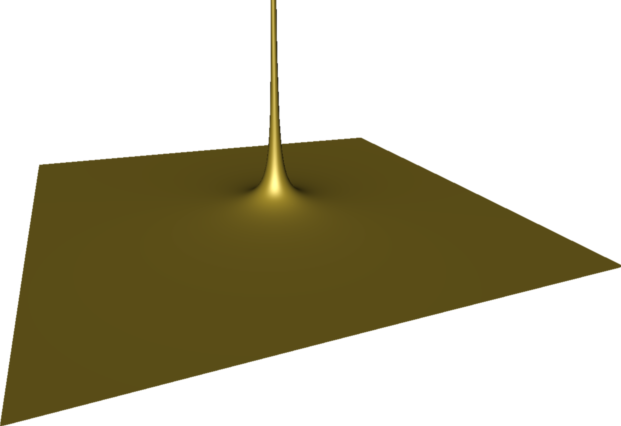
\includegraphics[align=c,width=0.29\textwidth]{f/shot_land.png}
\end{tabular}
\pause

%SCRIPT blur g 1 f/x.png o/x_g1.png
%SCRIPT blur g 15 f/x.png o/x_g15.png
%SCRIPT blur g 60 f/x.png o/x_g60.png
%SCRIPT fft 1 f/x.png|plambda ':R 1 ^ /'|ifft|qauto -i -p 0.1 - o/x_r1.png
%SCRIPT fft 1 f/x.png|plambda ':R 2 ^ /'|ifft|qauto -i -p 0.1 - o/x_r2.png
%SCRIPT fft 1 f/x.png|plambda ':R 3 ^ /'|ifft|qauto -i -p 0.1 - o/x_r3.png
%SCRIPT fft 1 f/x.png|plambda ':R -0.5 ^ /'|ifft|qauto -i -p 5 - o/x_rm05.png
%SCRIPT fft 1 f/x.png|plambda ':R -1 ^ /'|ifft|qauto -i -p 5 - o/x_rm1.png

\vspace{-1.5em}
\begin{center}
	\setlength{\tabcolsep}{1pt}
	\renewcommand{\arraystretch}{0.5}
	\begin{tabular}{ccccccc}
		\scriptsize $u$ &
		\scriptsize ${\color{darkblue}G_5} * u$ &
		\scriptsize ${\color{darkblue}G_{15}} * u$ &
		\scriptsize ${\color{darkblue}G_{60}} * u$ &
		\scriptsize ${\color{darkred}R_1} * u$ &
		\scriptsize ${\color{darkred}R_2} * u$ &
		\scriptsize ${\color{darkred}R_3} * u$ \\
		\includegraphics[width=0.14\textwidth]{f/x.png}&
		\includegraphics[width=0.14\textwidth]{o/x_g5.png}&
		\includegraphics[width=0.14\textwidth]{o/x_g15.png}&
		\includegraphics[width=0.14\textwidth]{o/x_g60.png}&
		\includegraphics[width=0.14\textwidth]{o/x_r1.png}&
		%\includegraphics[width=0.14\textwidth]{o/x_rm05.png}&
		%\includegraphics[width=0.14\textwidth]{o/x_rm1.png}\\
		\includegraphics[width=0.14\textwidth]{o/x_r2.png}&
		\includegraphics[width=0.14\textwidth]{o/x_r3.png}\\
	\end{tabular}
\end{center}

\end{frame}


% why is the gaussian kernel great (laplace quote)
\begin{frame}
WHY IS THE GAUSSIAN KERNEL SO NATURAL\\
=====================================

\end{frame}


% teaser snapshot (fake clouds)
\begin{frame}
SOME LIMITATIONS OF THE GAUSSIAN KERNEL\\
=======================================

\end{frame}


% plan
% 1. definition and properties of the Riesz semigroup
% 2. comparison with the Gaussian semigroup
% 3. applications
% 3.1. retinex
% 3.2. differentiable poisson editing
% 3.3. shepard interpolation
% 3.4. cloud simulation
\begin{frame}
OUTLINE\\
=======

1. Definition and properties of~$R_\sigma$ {\color{gray}(Riesz semigroup)}

2. Comparison with~$G_\sigma$ {\color{gray}(Gaussian semigroup)}

3. Applications in image processing\\
\color{gray}
$\quad$ 3.1. Really multi-scale Retinex\\
$\quad$ 3.2. Differentiable Poisson editing\\
$\quad$ 3.3. Inverse Distance Weighted interpolation\\
$\quad$ 3.4. Cloud simulation

\end{frame}


% definition and visualization, side by side
\begin{frame}
DEFINITION OF THE RIESZ KERNEL\\
==============================

\end{frame}


% fractional derivatives (as from wikipedia)
% [note: riesz kernel are fractional derivatives in dimension 2]
% https://en.wikipedia.org/wiki/Riemann%E2%80%93Liouville_integral
\begin{frame}
FRACTIONAL DERIVATIVES\\
======================

\end{frame}


% recall properties of fourier transform
\begin{frame}
PROPERTIES OF THE FOURIER TRANSFORM\\
===================================

\end{frame}


% definition in the spectral domain (by means of symmetries)
\begin{frame}
SPECTRUM OF THE RIESZ POTENTIAL\\
===============================

\end{frame}


% commutation with zoom
\begin{frame}
COMMUTATION WITH ZOOM\\
=====================

\end{frame}


% continuous interpolation between laplacian, retinex, image, blurry image
\begin{frame}
INTERESTING POINTS IN THE RIESZ SEMiGROUP\\
=========================================

\end{frame}


% first derivatives
\begin{frame}
GET FIRST DERIVATIVES FROM THE LAPLACIAN\\
========================================

\end{frame}


% closely related construction: riesz potentials, riesz transform
% https://en.wikipedia.org/wiki/Riesz_potential
% https://en.wikipedia.org/wiki/Riesz_transform
\begin{frame}
SIMILAR CONSTRUCTIoNS\\
=====================

\end{frame}

\begin{frame}
FORMAL DEFINITION, CONSTANTS\\
============================

\end{frame}


% the Land kernel (particular case for σ=1)
\begin{frame}
THE LAND KERNEL\\
===============

\end{frame}


% implementation: imscript (with fft), imscript (with blur), python
\begin{frame}
IMPLEMENTATION\\
==============

\end{frame}


% comparison table gauss/riesz/land
\begin{frame}
COMPARISON TABLE\\
================

\end{frame}




% 3. applications
\begin{frame}
APPLICATIONS\\
============

\end{frame}


% 3.1. multi-scale retinex (three-gaussians shit, are an approximation of land)
\begin{frame}
MULTI-SCALE RETINEX\\
===================

\end{frame}


% 3.2. - antilaplacian = land * land
\begin{frame}
ANTILAPLACIAN AND LAND\\
======================

\end{frame}


% 3.3. shepard interpolation
% https://en.wikipedia.org/wiki/Inverse_distance_weighting
\begin{frame}
shepard interpolation (idw)\\
===========================

\end{frame}


% 3.4. sobolev fractals, cloud simulation, other textures
\begin{frame}
SOBOLEV FRACTALS, CLOUD SIMULATION\\
==================================

\end{frame}


% gaussian mandelbrot quote
\begin{frame}
CLT AND ITS HEURISTIC CONVERSE\\
==============================

\end{frame}


% conclusion: links to slides, imscript, python function
\begin{frame}
CONCLUSIOn\\
==========

\end{frame}


% colophon: makefile that runs experiments and builds everything
\begin{frame}
COLOPHON\\
========

\end{frame}


\end{document}


% vim:sw=2 ts=2 spell spelllang=en:
